\RequirePackage{ifpdf}
\documentclass[letterpaper,landscape]{slides}
%\documentclass[letterpaper,portrait]{slides}
\usepackage{boxedminipage}
\usepackage{amsmath}
\usepackage{amssymb}
\usepackage{bm}

%\input /u/rhl/TeX/pdf.tex
\input pdf.tex

\newif\ifTalk\Talktrue		% We generating a talk, not printing
%\Talkfalse			% no; we're really printing

%\pagestyle{empty}
\setlength{\topmargin}{-1in}
\setlength{\textheight}{7.5in}
\setlength{\textwidth}{9in}
\setlength{\oddsidemargin}{0pt}
\setlength{\oddsidemargin}{0pt}

%\onlyslides{1-3,4,10-9999}
%\onlyslides{26-9999}

\begin{document}

\newcommand{\XXX}[1]{\textbf{XXX} #1}
\newcommand{\colour}[1]{\color{#1}}

\def\eq#1{\begin{equation} \color{blue} #1 \end{equation}}
\def\vx{{\bf x}}
\def\vv{{\bf v}}
\def\p{\partial}
\def\b#1{{\bf  #1}}
\def\p{\partial}
\def\th{^{th}}
\def\msun{{\rm\,M_\odot}}
\def\bnabla{{\bf\nabla}}
\def\dint{\int\!\!\!\int}
\def\d{{\rm d}}
\def\i{{\rm i}}
\def\ddt#1{{\rm{d} #1\over {\rm dt}}}
\def\ddtS#1{{\rm{d^2} #1\over {\rm dt^2}}}
%\lta and \gta produce > and < signs with twiddle underneath
\def\spose#1{\hbox to 0pt{#1\hss}}
\def\lta{\mathrel{\spose{\lower 3pt\hbox{$\mathchar"218$}}
     \raise 2.0pt\hbox{$\mathchar"13C$}}}
\def\gta{\mathrel{\spose{\lower 3pt\hbox{$\mathchar"218$}}
     \raise 2.0pt\hbox{$\mathchar"13E$}}}
\def\mspace{\hbox{\quad}}
\def\deffn#1{{\bf#1}}\def\eqs#1{equations \rf#1}






\newcount\itemCnt\itemCnt=0
\newcommand{\nitem}{%
  \global\advance\itemCnt by 1
  ~\vskip0cm\the\itemCnt.\qquad}

\definecolor{orange}{rgb}{1.0, 0.5, 0.0}
\definecolor{purple}{cmyk}{0.4, 0.8, 0.3, 0.0}


%%%%%%%%%%%%%%%%%%%%%%%%%%%%%%%%%%%
\newcommand{\onepic}[6]{%
\begin{slide}
     \begin{center}
        \begin{minipage}{#1in}
            {\large \color{blue} #6}
            \phantom{x} \vskip #2in
            \phantom{x} \hskip #3in
            {\scalebox{#4}{\includegraphics{#5}}}   
        \end{minipage}
     \end{center}
    \vfill
\end{slide}
}


%%%%%%%%%%%%%%%%%%%%%%%%%%%%%%%%%%%
\newcommand{\picslide}[7]{%
  \begin{slide}
     \begin{center}
        \begin{minipage}{#5in}
            \hskip #6in
            \hskip -1in
            {\scalebox{#4}{\includegraphics{#1.#2}}}
            \vskip #7in~
            {\large \color{blue} #3}
        \end{minipage}
     \end{center}
     \vfill
  \end{slide}
}
%%%%%%%%%%%%%%%%%%%%%%%%%%%%%%%%%%%
 

%%%%%%%%%%%%%%%%%%%%%%%%%%%%%%%%%%%
\newcommand{\Spicslide}[7]{%
  \begin{slide}
     \begin{center}
        \begin{minipage}{#5in}
            \vskip #6in
            \hskip #7in
            {\scalebox{#4}{\includegraphics{#1.#2}}}
        \end{minipage}
     \end{center}
     \vfill
  \end{slide}
}
%%%%%%%%%%%%%%%%%%%%%%%%%%%%%%%%%%%
 



%------------------------------------------------------------------------------

\begin{slide}

\phantom{x}
\vskip -2in
\begin{center}
\bfseries
{\large {\color{blue} Astr 511: Galaxies as galaxies}}
\end{center}

{\centerline {{\color{blue} 
Winter Quarter 2017, University of Washington}}}
{\centerline {{\color{blue} 
Mario Juri\'{c} \& \v{Z}eljko Ivezi\'{c} }}}

\vskip 1.6in

{\centerline {\huge {\color{red}      Lecture 12:             }}}
\vskip 0.2in 
{\centerline {\Large {\color{blue} Stellar count distribution in }}}
\vskip 0.1in
{\centerline {\Large {\color{blue} the Milky Way  }}}

\vfill
\end{slide}
%------------------------------------------------------------------------------



%------------------------------------------------------------------------------
\Spicslide{figures/MWmarioDM}{jpg}{}{0.90}{7}{-0.48}{-2.45} 
%------------------------------------------------------------------------------


%------------------------------------------------------------------------------
% TWO-SIDED PAGE 
\begin{slide}

\hbox to \hsize{
\begin{minipage}[t]{16cm}
\begin{center}
\vskip -1.7in
\scalebox{0.4}{\hskip -3.3in \includegraphics{figures/MW_Poster18x24_noText.pdf}}

\end{center}

\end{minipage}

\begin{minipage}[t]{8cm}
\begin{center}
{\large \color{red} The three basic stellar distribution functions:}
\end{center}
\vskip 0.3in
\begin{enumerate}
\item {\bf Number density}
\item  {\bf Metallicity}
\item  {\bf Kinematics} 
\end{enumerate}     

{\large \color{blue} These three distribution functions provide
observational constraints for the model selection} (models for
galaxy formation and evolution)


\end{minipage}}
\vfill 
\end{slide}
%------------------------------------------------------------------------------




%------------------------------------------------------------------------------
\begin{slide}
\begin{center}
{\color{red}               Galaxy Formation Scenarios (abridged)}
\end{center}

{\color{blue} The ELS Monolithic Collapse Model}

\begin{itemize}
\item The ELS model (Eggen, Lynden-Bell and Sandage, 1962):
the Milky Way formed from the rapid collapse of a large proto-galactic 
nebula:  {\color{blue} top-down scenario}
\item Searle \& Zinn (1978): galaxies are built up from 
        merging smaller fragments: {\color{blue} a bottom-up scenario} 
\end{itemize}

\scalebox{0.9}{\hskip  1.1in \includegraphics{figures/motion.jpg}}
%\vskip -0.1in
\scalebox{0.6}{\hskip  0.5in \includegraphics{figures/formation.jpg}}


\vfill
\end{slide}

%------------------------------------------------------------------------------


%------------------------------------------------------------------------------
\begin{slide}
{\color{red} Problems with the ELS collapse scenario:}
\vskip -0.5in
\begin{itemize}
      \item {\color{blue} Why are half the halo stars in retrograde orbits?} We would
        expect that most stars would be moving in roughly the same direction (on highly
        elliptical orbits) because of the initial rotation of the proto-Galactic cloud.
      \item {\color{blue} Why there is an age spread of $\sim$ 3 Gyr among globular clusters (GCs)?} 
        We would expect $<1$ Gyr spread (free-fall time).
\end{itemize}
{\color{red} Some important questions that are left without robust answers:}
\vskip -0.5in
\begin{itemize}
      \item {\color{blue} Why GCs become more metal-poor with the distance from the center?}
%      \item {\color{blue} Why there are two disks with different ages?}          
      \item{\color{blue}  Detailed calculations of chemical enrichment predict about 10 times
                          too many metal-poor stars in the solar neighborhood (the G-dwarf problem), why?}
\end{itemize}
\vfill
\end{slide}

%------------------------------------------------------------------------------



%------------------------------------------------------------------------------
\begin{slide}
\begin{center}
{\color{red}  Which model for galaxy formation is correct (or less wrong)?}
\end{center}
  
\begin{itemize}
\item by observing galaxies at large redshifts (beyond 1), we are probing 
      the epoch of galaxy formation -- indeed, {\color{blue}  galaxies at large redshifts
      have very different morphologies}, and the fraction of spirals in 
      clusters is greater than today (Butcher-Oemler effect). Also, {\color{blue}  the
      volume density of galaxies was larger in the past}: appears consistent with
      the bottom-up approach
\item {\color{red} We have some important detailed evidence for galaxy merging in our 
    own backyard:} the Milky Way structure and kinematics
\item {\color{blue} How smooth, or clumpy, is the distribution of stars and their kinematics
   in the Milky Way?}
\end{itemize}
\vfill
\end{slide}
%------------------------------------------------------------------------------





%------------------------------------------------------------------------------
\begin{slide}
\begin{center}
\bfseries
{\large {\color{blue} The Milky Way Structure,} as seen by SDSS}
\end{center}
\vskip -0.3in

\begin{enumerate}
             \item Spatial Distribution of Stars
             \item Metallicity Distribution
             \item Stellar Kinematics 
\end{enumerate}

{\color{red} Advantages of SDSS for studying the Milky Way structure}
   \begin{itemize}
   \item {\color{blue} Accurate photometry:} distance and [Fe/H] estimates
   \item {\color{blue} Numerous stars:} small random errors for number density
   \item {\color{blue} Large area and faint limit}: good volume coverage 
   \end{itemize}

\vfill
\end{slide}
 
%------------------------------------------------------------------------------





%------------------------------------------------------------------------------
% TWO-SIDED PAGE 
\begin{slide}

\hbox to \hsize{
\begin{minipage}[t]{8cm}
\begin{center}
\vskip -0.45in
\scalebox{0.45}{\hskip -1.85in \includegraphics{figures/SgrPlane.jpg}}
\end{center}
\end{minipage}

\begin{minipage}[t]{16cm}
\begin{itemize}
\item SDSS RR Lyrae and other luminous tracers, and 2MASS M giants, demonstrate that 
      {\color{red} the Milky Way halo extends to $\sim$100 kpc and has a lot of substructure}
\item The color-coded map of RR Lyrae density (times $R^3$) uses a Bayesian density
       estimator from Ivezi\'{c} et al. (2005).
\item The map below is from Belokurov et al. (2007)  ($\sim$10 kpc scales)  
\end{itemize}     

\vskip 0.7in
\scalebox{0.5}{\hskip -1.0in \includegraphics{figures/field_of_streams.jpg}} 

\end{minipage}}
\vfill 
\end{slide}
%------------------------------------------------------------------------------




%------------------------------------------------------------------------------
% TWO-SIDED PAGE 
\begin{slide}

\hbox to \hsize{
\begin{minipage}[t]{8cm}
\begin{center}
\vskip -0.45in
\scalebox{0.45}{\hskip -1.85in \includegraphics{figures/SgrPlane.jpg}}
\vskip 0.5in
{\color{blue}
\begin{eqnarray}
              n_o = { C  \over \sum_{i=1}^N d_i^D}  \nonumber
\end{eqnarray}
}
\vskip 0.2in
where $C$ can be estimated by requiring $<n_o> = N_{tot}/V_{tot}$. 
\end{center}
\end{minipage}

\begin{minipage}[t]{16cm}
\centerline{\color{blue} \bf Density traced by a point distribution}
\begin{itemize}
\item Given N points distributed in D-dimensional space, the volume number
density, $n_o$, can estimated using the distance to the $N$th nearest neighbor
as
\begin{eqnarray}
                  n_o = { N  \over V_D(d_N)}, \nonumber
\end{eqnarray}
where $V_D(d)$ is evaluated according to the problem dimensionality, $D$ 
(for $D=3$, $V_3(d)=4\pi d^3/3$, and $V_2=\pi d^2$ for $D=2$).
\item
More generally, distances to {\it all} $N$ nearest neighbors contain
information about the local density, and this information can be easily 
incorporated into a density estimator within the Bayesian probability
framework. Following Ivezi\'{c} et al. (2005, AJ 129, 1096; see Appendix B),
see left.
\item
{\color{red} More density estimation methods can be found in astroML! }
\end{itemize}     

\end{minipage}}
\vfill 
\end{slide}
%------------------------------------------------------------------------------


%------------------------------------------------------------------------------
% TWO-SIDED PAGE 
\begin{slide}

\hbox to \hsize{
\begin{minipage}[t]{5cm}
\begin{center}
\vskip -0.45in
\scalebox{0.85}{\hskip -1.25in \includegraphics{figures/bayes1.jpg}}
\end{center}
\end{minipage}

\begin{minipage}[t]{19cm}
\centerline{\color{blue} \bf Density traced by a point distribution}
\begin{itemize}
\item $n_o$ is the {\it mean} density, however, the method gives the full 
posterior probability distribution
for the local density
\begin{eqnarray}
  p(d_o|\{d_k; k=1,N\}) \propto 
    \prod_{k=1}^{N} \, {2 {\rm e}^{-(d_k/d_o)^2} \over d_o\, (k-1)!} \,
    \left({d_k \over d_o}\right)^{2k-1} \nonumber
\end{eqnarray}
where $n_o=\pi \, d_o^2$.
\item {\bf Left:} The {\bf top} shows the $k^{\rm th}$ nearest neighbor (NN) 
distance distribution, $k$=2, 4 and 8, for a random 2-dim. sample. 
The {\bf middle} panel displays the evolution of the posterior
probability density distribution, $p(d_o|...)$, for a sample with true $d_o=1$.
The dashed line in the {\bf bottom} panel shows a typical $p(d_o|...)$
based on only the 8th NN in a random sample with $d_o=1$. The dot-dashed curve 
shows $p(d_o|...)$ based on all 7 nearest neighbors. This distribution is 
used as the prior to evaluate the final $p(d_o|...)$ based on all 8 NN 
(solid line).
\end{itemize}     

\end{minipage}}
\vfill 
\end{slide}
%------------------------------------------------------------------------------



%------------------------------------------------------------------------------
% TWO-SIDED PAGE 
\begin{slide}

\hbox to \hsize{
\begin{minipage}[t]{8cm}
\begin{center}
\vskip -0.45in
\scalebox{0.45}{\hskip -1.85in \includegraphics{figures/SgrPlane.jpg}}
\end{center}
\end{minipage}

\begin{minipage}[t]{16cm}
\begin{itemize}
\item SDSS RR Lyrae and other luminous tracers, and 2MASS M giants, demonstrate that 
      {\color{red} the Milky Way halo extends to $\sim$100 kpc and has a lot of substructure}
\item {\color{blue} SDSS has obtained excellent photometric data for over
    100 million stars.}  
      How can one utilize these data for studying the disk component?
\item {\color{red} What is the structure of the disk component, including 
    kinematics and metallicity distributions?}
\end{itemize}     

\vskip 0.1in
\scalebox{0.045}{\hskip -55.4in 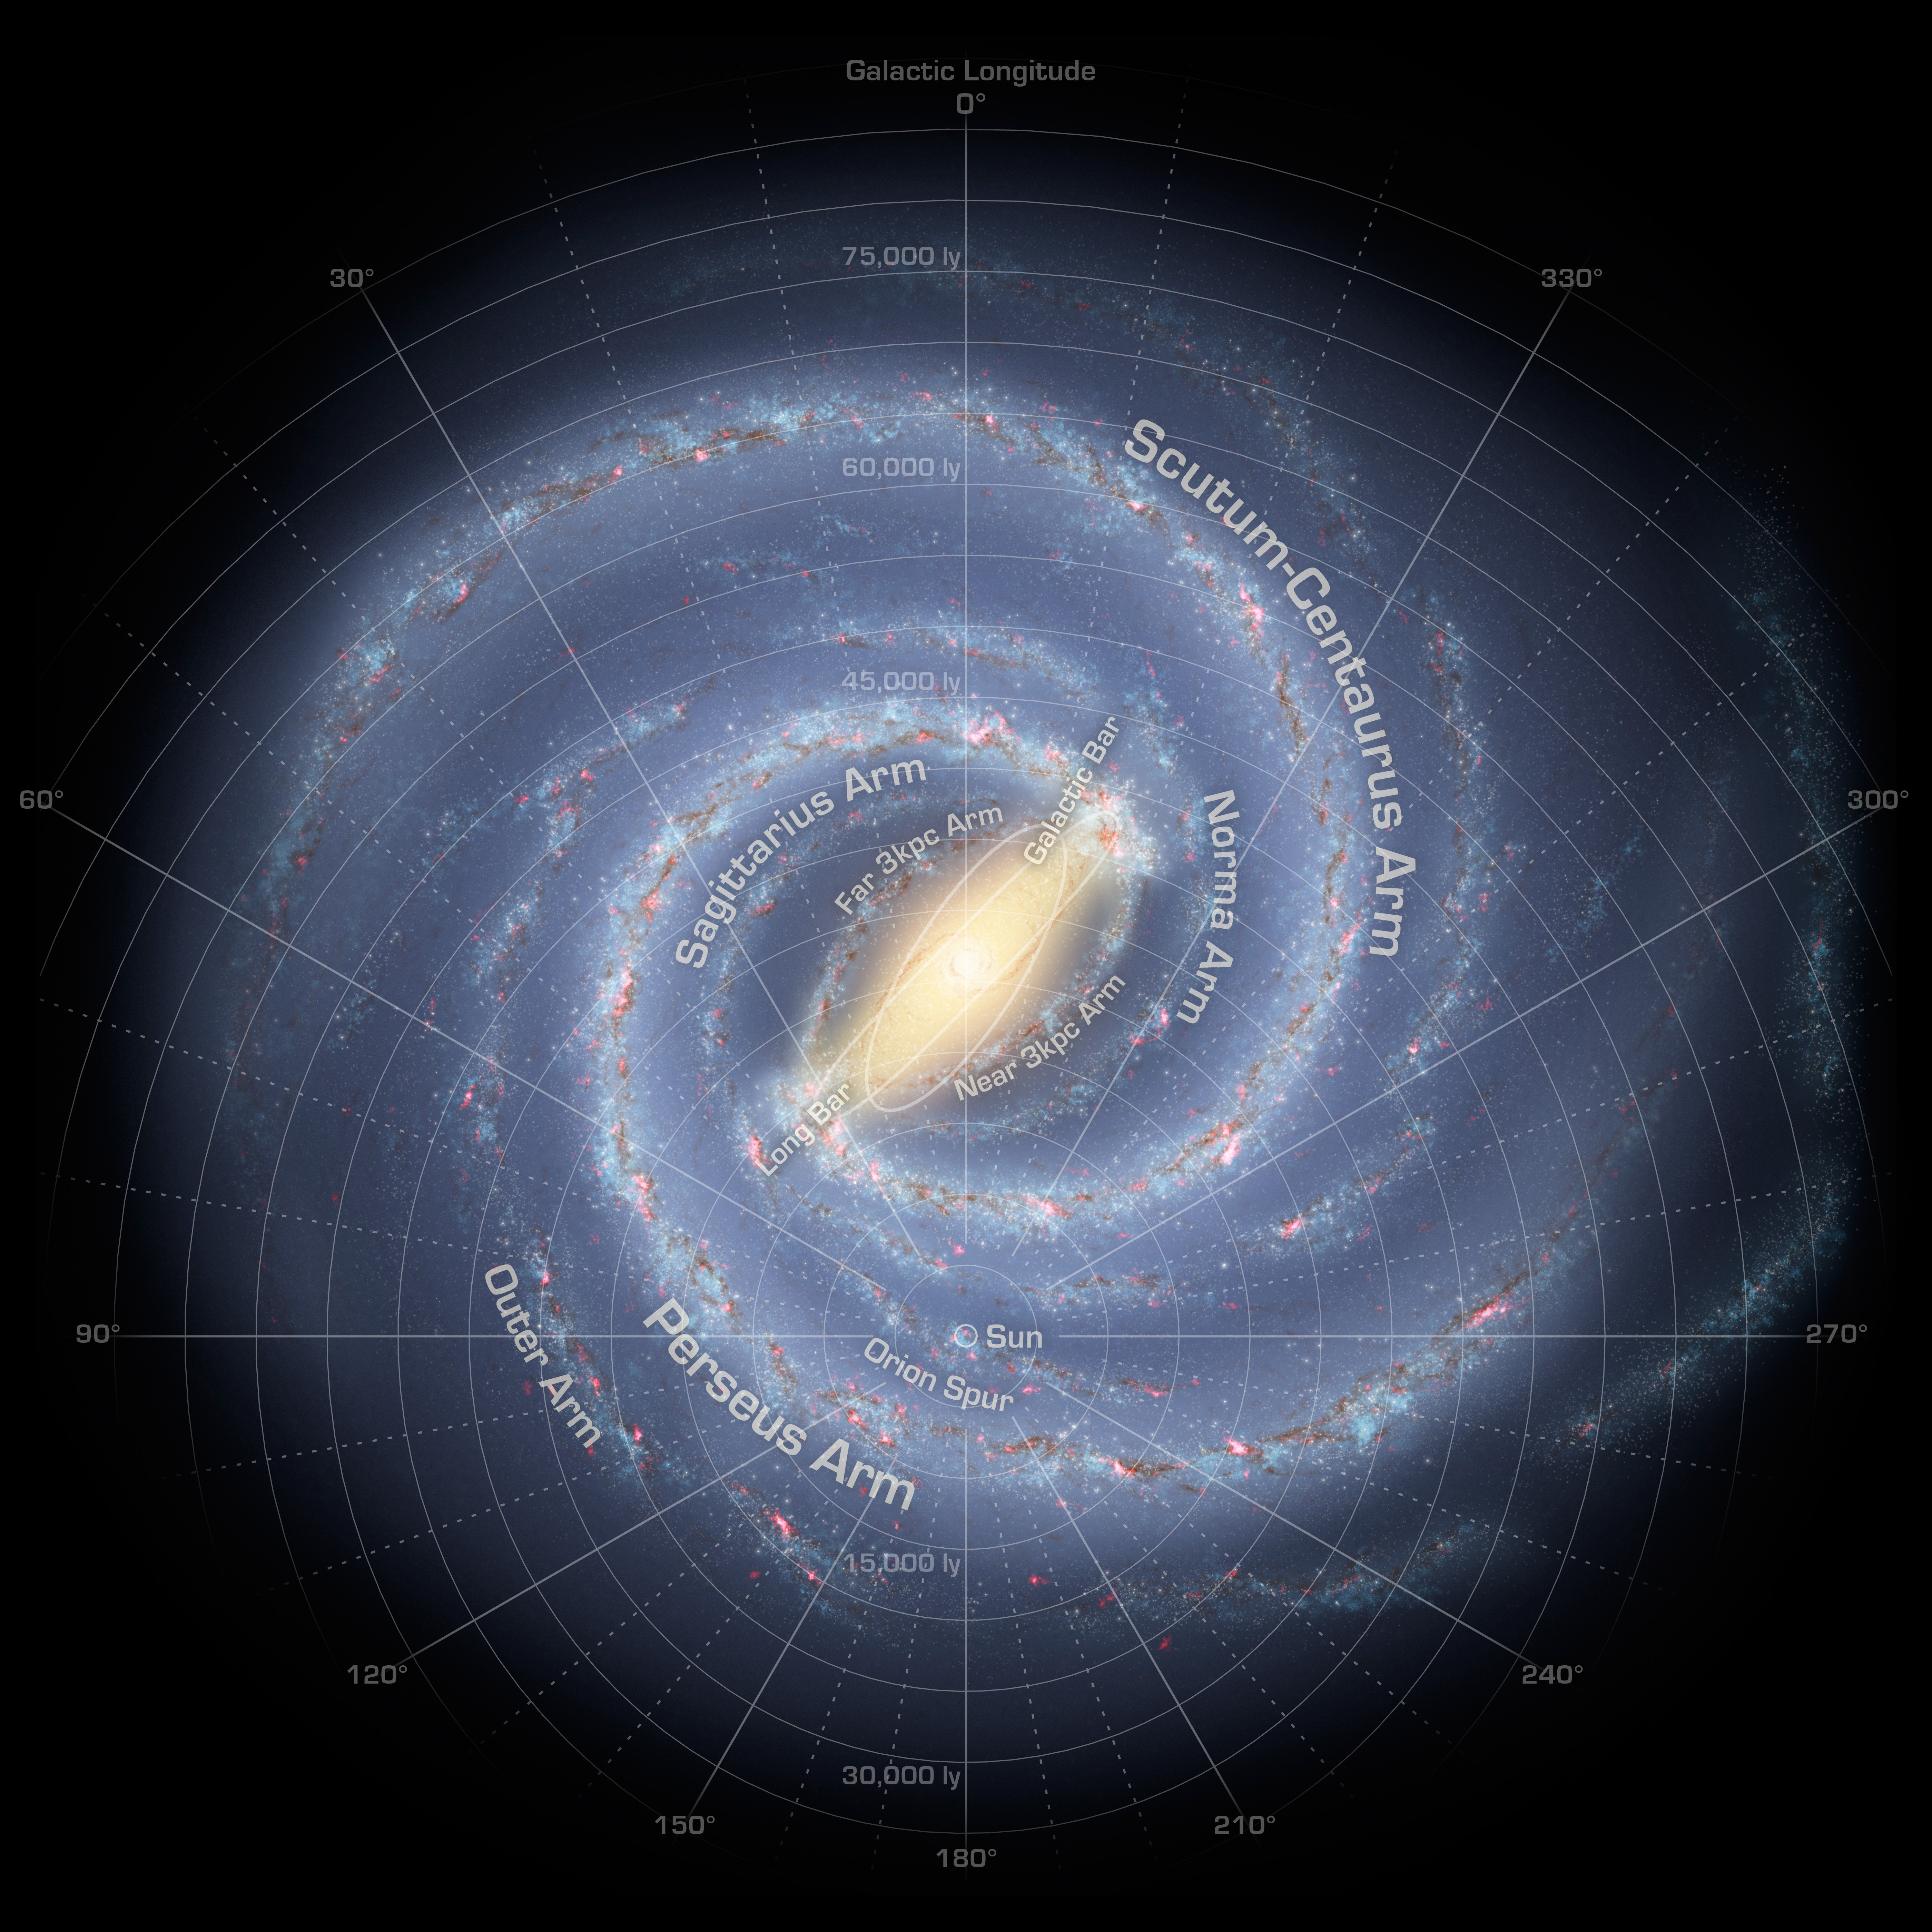
\includegraphics{figures/MWplaneAnnotated.jpg}}
\scalebox{0.36}{\hskip 1.7in \includegraphics{figures/MilkyWay2.jpg}} 

\end{minipage}}
\vfill 
\end{slide}
%------------------------------------------------------------------------------





%------------------------------------------------------------------------------
% TWO-SIDED PAGE 
\begin{slide}

\hbox to \hsize{
\begin{minipage}[t]{0.001cm}
\begin{center}
\vskip -0.2in
%\scalebox{0.61}{\hskip -1.7in \includegraphics{figures/modelsdiskshalo.jpg}}
\end{center}
\end{minipage}

\begin{minipage}[t]{23cm}
\begin{center}
\vskip -1in
{\large \color{red} Constraining Thin/Thick Disk$+$Halo Models}
\end{center}
\begin{itemize}
\item
{\color{red} Observationally,} $\rho(z|R=R_\odot)$ is well fit by {\color{blue} 
a sum of double  
% \,\,\,\,\,  \,\,\,\,\,
 exponential (thin and thick disk) and power-law} profiles. 
\item
However, {\bf the best-fit models are degenerate:} {\color{blue} e.g. the
thick 
% \,\,\,\,\,
disk scale height varies by a factor of few and its normalization 
by an order 
of magnitude!}
\end{itemize}     
\vskip 0.1in
\scalebox{0.38}{\hskip -3.0in \includegraphics{figures/rhoZdiskshalo.jpg}}
\vskip -3.6in
\scalebox{0.62}{\hskip 5.8in \includegraphics{figures/siegel.jpg}}

\vskip -4.8in 
{\color{red} \hskip -0.2in THIN}

\vskip 0.9in
{\color{blue} \hskip 1.6in HALO}

\vskip 0.1in
{\color{red} \hskip -0.0in THICK}

\end{minipage}}
\vfill 
\end{slide}
%------------------------------------------------------------------------------

%------------------------------------------------------------------------------
% TWO-SIDED PAGE 
\begin{slide}

\hbox to \hsize{
\begin{minipage}[t]{4cm}
\begin{center}
\vskip -0.2in
\scalebox{0.61}{\hskip -1.7in \includegraphics{figures/modelsdiskshalo.jpg}}
\end{center}
\end{minipage}

\begin{minipage}[t]{20cm}
\begin{center}
\vskip -1in
{\large \color{red} Constraining Thin/Thick Disk$+$Halo Models}
\end{center}
\begin{itemize}
\item
{\color{red} Observationally,} $\rho(z|R=R_\odot)$ is well fit by {\color{blue} 
a sum of double exponential (thin and thick disk) and power-law} profiles. 
\item
But, very {\color{blue} different models} (top: thin and thick disk 
without halo; middle: single disk and halo, bottom: the difference) {\color{blue} 
can produce the same $\rho(z|R=R_\odot)$}
\item
{\color{blue}A large sky area is needed to break model degeneracies} (pencil
beam surveys are inconclusive)
\item {\color{red} SDSS is the first survey with the required data}
\end{itemize}     
\vskip 0.1in
\scalebox{0.41}{\hskip 0.8in \includegraphics{figures/rhoZdiskshalo.jpg}}

\end{minipage}}
\vfill 
\end{slide}
%------------------------------------------------------------------------------



%------------------------------------------------------------------------------
% TWO-SIDED PAGE 
\begin{slide}

\hbox to \hsize{
\begin{minipage}[t]{9cm}
\begin{center}
\vskip -0.7in
\scalebox{0.9}{\hskip -0.7in \includegraphics{figures/ppMetal.jpg}}

\end{center}

\end{minipage}

\begin{minipage}[t]{13cm}
\begin{center}
\vskip -1in
{\large {\color{red} Photometric Distance and Photometric [Fe/H]}: reminder}
\end{center}

\begin{itemize}
\item
Determined absolute magnitude vs. color vs. metallicity relation
using globular clusters observed by SDSS (blue end), and nearby 
stars with trigonometric parallaxes (red end)
\item 
{\color{blue} The $g-i$ color of a main-sequence star constrains its
absolute magnitude to within 0.1-0.2 mag} (0.3 mag for unresolved
binaries), assuming [Fe/H] is known
\end{itemize}     

\end{minipage}}
\vfill 
\end{slide}
%------------------------------------------------------------------------------


%------------------------------------------------------------------------------
% TWO-SIDED PAGE 
\begin{slide}

\hbox to \hsize{
\begin{minipage}[t]{9cm}
\begin{center}
\vskip -0.7in
\scalebox{0.9}{\hskip -0.7in \includegraphics{figures/ppMetal.jpg}}
\vskip -4.0in
\scalebox{0.5}{\hskip -1.2in \includegraphics{figures/ugrMetal.jpg}}
\end{center}

\end{minipage}

\begin{minipage}[t]{13cm}
\begin{center}
\vskip -1in
{\large {\color{red} Photometric Distance and Photometric [Fe/H]}: reminder}
\end{center}

\begin{itemize}
\item
Determined absolute magnitude vs. color vs. metallicity relation
using globular clusters observed by SDSS (blue end), and nearby 
stars with trigonometric parallaxes (red end)
\item 
{\color{blue} The $g-i$ color of a main-sequence star constrains its
absolute magnitude to within 0.1-0.2 mag} (0.3 mag for unresolved
binaries), assuming [Fe/H] is known 
\item For F and G stars ($0.2<g-r<0.6$), accurate SDSS $u-g$ color
measurements enable {\color{blue} photometric metallicity estimates 
as precise (0.1-0.2 dex) as [Fe/H] derived from SDSS spectra} 
\end{itemize}     

\end{minipage}}
\vfill 
\end{slide}

%------------------------------------------------------------------------------

\begin{slide}
\begin{center}
{\large \color{red}  Dissecting Milky Way with SDSS}
\end{center}

{\bf \color{blue} Good ugriz photometry gives decent distance (and metallicity)
estimates for PRACTICALLY EVERY SINGLE STAR within areal and flux 
(and color) limits, and greatly simplifies the data analysis:}

\begin{itemize}
\item
{\color{red} Traditional approach:} assume initial mass function, fold with 
models for stellar evolution; assume mass-luminosity relation;
assume some parametrization for the number density distribution;
vary (numerous) free parameters until the observed and model
counts agree. {\color{blue} Uniqueness? Validity of all
assumptions?} 
\item
{\color{red} SDSS photometric parallax  approach:} adopt color-luminosity
relation, estimate distance to each star, bin the stars in XYZ space
and directly compute the stellar number density (for each narrow color bin). 
{\color{blue} There is no need to a priori assume, the number of, and analytic form
for Galactic components}
\end{itemize}  

\vfill
\end{slide}

%------------------------------------------------------------------------------



%------------------------------------------------------------------------------
% TWO-SIDED PAGE 
\begin{slide}

\hbox to \hsize{
\begin{minipage}[t]{9cm}
\begin{center}
\vskip -0.2in
%\scalebox{0.75}{\hskip -0.9in \includegraphics{figures/juric3.jpg}}
\scalebox{0.45}{\hskip -0.9in \includegraphics{figures/coordEx.jpg}}
\vskip 0.5in
\scalebox{0.6}{\hskip -2.05in \includegraphics{figures/redRZrho.jpg}}
\vskip -7.1in 
{\color{blue} \hskip 0.65in \bf o}

\end{center}
\end{minipage}

\begin{minipage}[t]{13cm}
\begin{center}
\vskip -1in
{\large \color{red} Local maps: thin disk}
\end{center}

\begin{itemize}
\item Red(ish) stars have small luminosity: sampled to a few kpc
\item {\color{blue} Out to $\sim$1 kpc, the maps are roughly consistent 
with an exponential disk:} the lines of constant density are straight lines
\item The slope of these lines is given by the ratio of exponential
scale height and scale length 
\end{itemize}     
\vskip 0.1in
\scalebox{0.56}{\hskip 0.7in \includegraphics{figures/juric7a.jpg}}

\end{minipage}}
\vfill 
\end{slide}
%------------------------------------------------------------------------------



%------------------------------------------------------------------------------
\begin{slide}

\begin{center}
\vskip -0.6in
\scalebox{0.75}{\hskip -0.9in \includegraphics{figures/MW_ri_scales.jpg}}
\end{center}


\vfill
\end{slide}

%------------------------------------------------------------------------------




%------------------------------------------------------------------------------
% TWO-SIDED PAGE 
\begin{slide}

\hbox to \hsize{
\begin{minipage}[t]{8cm}
\begin{center}
\vskip 0.1in
\scalebox{0.8}{\hskip -1.25in \includegraphics{figures/marioRZ1.jpg}}

\end{center}
\end{minipage}

\begin{minipage}[t]{16cm}
\begin{center}
\vskip -1in
{\large \color{red} Dissecting the Milky Way with SDSS }
\end{center}
\vskip -0.4in

\begin{itemize}
\item Juri\'{c} et al. 2008 (ApJ 673, 864): {\color{blue} unprecedented 
panoramic view of the Milky Way, akin to observations of external galaxies;}
with exceedingly high signal-to-noise.
\end{itemize}     
\vskip -0.3in
\scalebox{0.45}{\hskip 2.9in \includegraphics{figures/J08models0.jpg}}
\vskip -0.05in
\scalebox{0.45}{\hskip 2.7in \includegraphics{figures/J08models2.jpg}}

\end{minipage}}
\vfill 
\end{slide}
%------------------------------------------------------------------------------



%------------------------------------------------------------------------------
% TWO-SIDED PAGE 
\begin{slide}

\hbox to \hsize{
\begin{minipage}[t]{6cm}
\begin{center}
\vskip -0.8in
\scalebox{1.0}{\hskip -0.7in \includegraphics{figures/J08counts.jpg}}

\end{center}
\end{minipage}

\begin{minipage}[t]{17cm}
\begin{center}
\vskip -1in
{\large \color{red} Dissecting the Milky Way with SDSS }
\end{center}

\begin{itemize}
\item Panoramic view of the Milky Way:
{\color{blue} good support for standard Galactic models:}
\end{itemize}     
\vskip 0.25in
\scalebox{0.55}{\hskip -0.2in \includegraphics{figures/MWmodels.jpg}}
\vskip 0.1in
\scalebox{0.65}{\hskip 1.7in \includegraphics{figures/siegel2.jpg}}
\vskip -4.25in
{\color{red} \bf \hskip 1.7in SDSS}
\end{minipage}}
\vfill 
\end{slide}
%------------------------------------------------------------------------------


%------------------------------------------------------------------------------
% TWO-SIDED PAGE 
\begin{slide}

\hbox to \hsize{
\begin{minipage}[t]{6cm}
\begin{center}
\vskip -0.8in
\scalebox{1.0}{\hskip -0.7in \includegraphics{figures/J08counts.jpg}}

\end{center}
\end{minipage}

\begin{minipage}[t]{17cm}
\begin{center}
\vskip -1in
{\large \color{red} Dissecting the Milky Way with SDSS }
\end{center}

\begin{itemize}
\item Panoramic view of the Milky Way:
{\color{blue} good support for standard Galactic models}
\item
{\color{red} Are we overfitting data with two disks and a halo?} 
\item
{\color{blue} Metallicity mapping} supports components inferred 
from number counts mapping:
\end{itemize}     
\vskip 0.3in
\scalebox{0.6}{\hskip 2.0in \includegraphics{figures/FeHmapNGP.jpg}}

\end{minipage}}
\vfill 
\end{slide}
%------------------------------------------------------------------------------
%------------------------------------------------------------------------------
% TWO-SIDED PAGE 
\begin{slide}

\hbox to \hsize{
\begin{minipage}[t]{6cm}
\begin{center}
\vskip -0.8in
\scalebox{1.0}{\hskip -0.7in \includegraphics{figures/J08counts.jpg}}

\end{center}
\end{minipage}

\begin{minipage}[t]{17cm}
\begin{center}
\vskip -1in
{\large \color{red} Dissecting the Milky Way with SDSS }
\end{center}

\begin{itemize}
\item {\color{blue} SDSS count maps provide good support for standard 
Galactic models}
\item
However, the subtraction of (conventional) best-fit model maps from the 
data maps reveals {\color{blue} rich substructure} 
\item The number count excess is typically 20-40\% -- not easy to
see with older data!
\end{itemize}  
%  \vskip 0.1in
\vskip 0.1in
\scalebox{0.45}{\hskip 3.9in \includegraphics{figures/DR5_ex1.jpg}}
\vskip -4.8in
{\color{red} $\rm{The \,\, Virgo \,\, overdensity}$}

\end{minipage}}
\vfill 
\end{slide}
%------------------------------------------------------------------------------


%------------------------------------------------------------------------------
% TWO-SIDED PAGE 
\begin{slide}

\hbox to \hsize{
\begin{minipage}[t]{6cm}
\begin{center}
\vskip -0.5in
\scalebox{0.85}{\hskip 0.1in \includegraphics{figures/marioRZ3.jpg}}

\end{center}
\end{minipage}

\begin{minipage}[t]{17cm}
\begin{center}
%{\large \color{red} Dissecting the Milky Way with SDSS }
\end{center}

\end{minipage}}
\vfill 
\end{slide}
%------------------------------------------------------------------------------


%------------------------------------------------------------------------------
% TWO-SIDED PAGE 
\begin{slide}

\hbox to \hsize{
\begin{minipage}[t]{6cm}
\begin{center}
\vskip -0.5in
\scalebox{0.9}{\hskip 0.1in \includegraphics{figures/marioRZ2.jpg}}

\end{center}
\end{minipage}

\begin{minipage}[t]{17cm}
\begin{center}
%{\large \color{red} Dissecting the Milky Way with SDSS }
\end{center}

\end{minipage}}
\vfill 
\end{slide}
%------------------------------------------------------------------------------

%------------------------------------------------------------------------------
% TWO-SIDED PAGE 
\begin{slide}

\hbox to \hsize{
\begin{minipage}[t]{1cm}
\begin{center}
\vskip 2.9in
\scalebox{0.8}{\hskip -0.9in \includegraphics{figures/SgrStreamPanoramic_Casey2012.jpg}}
\end{center}
\end{minipage}

\begin{minipage}[t]{20cm}
\begin{center}
\vskip -1in
{\large \color{red} The Virgo Overdensity: the latest news}
\end{center}
\vskip 0.2in
\begin{itemize}
\item ``...the Virgo Overdensity ... is best explained by a minor merger.''
(Bonaca et al. 2012, AJ 143, 105), 
\item
``... a tri-axial dark matter halo is favored and we exclude a prolate shape.''
(Casey, Keller \& Da Costa 2012, AJ 143, 88; figure below is from this paper)
\end{itemize}  


\end{minipage}}
\vfill 
\end{slide}
%--------------------------------------------------------------------------------------------


%------------------------------------------------------------------------------
% TWO-SIDED PAGE 
\begin{slide}

\hbox to \hsize{
\begin{minipage}[t]{10cm}
\begin{center}
\vskip -0.75in
\scalebox{0.05}{\hskip -10.4in 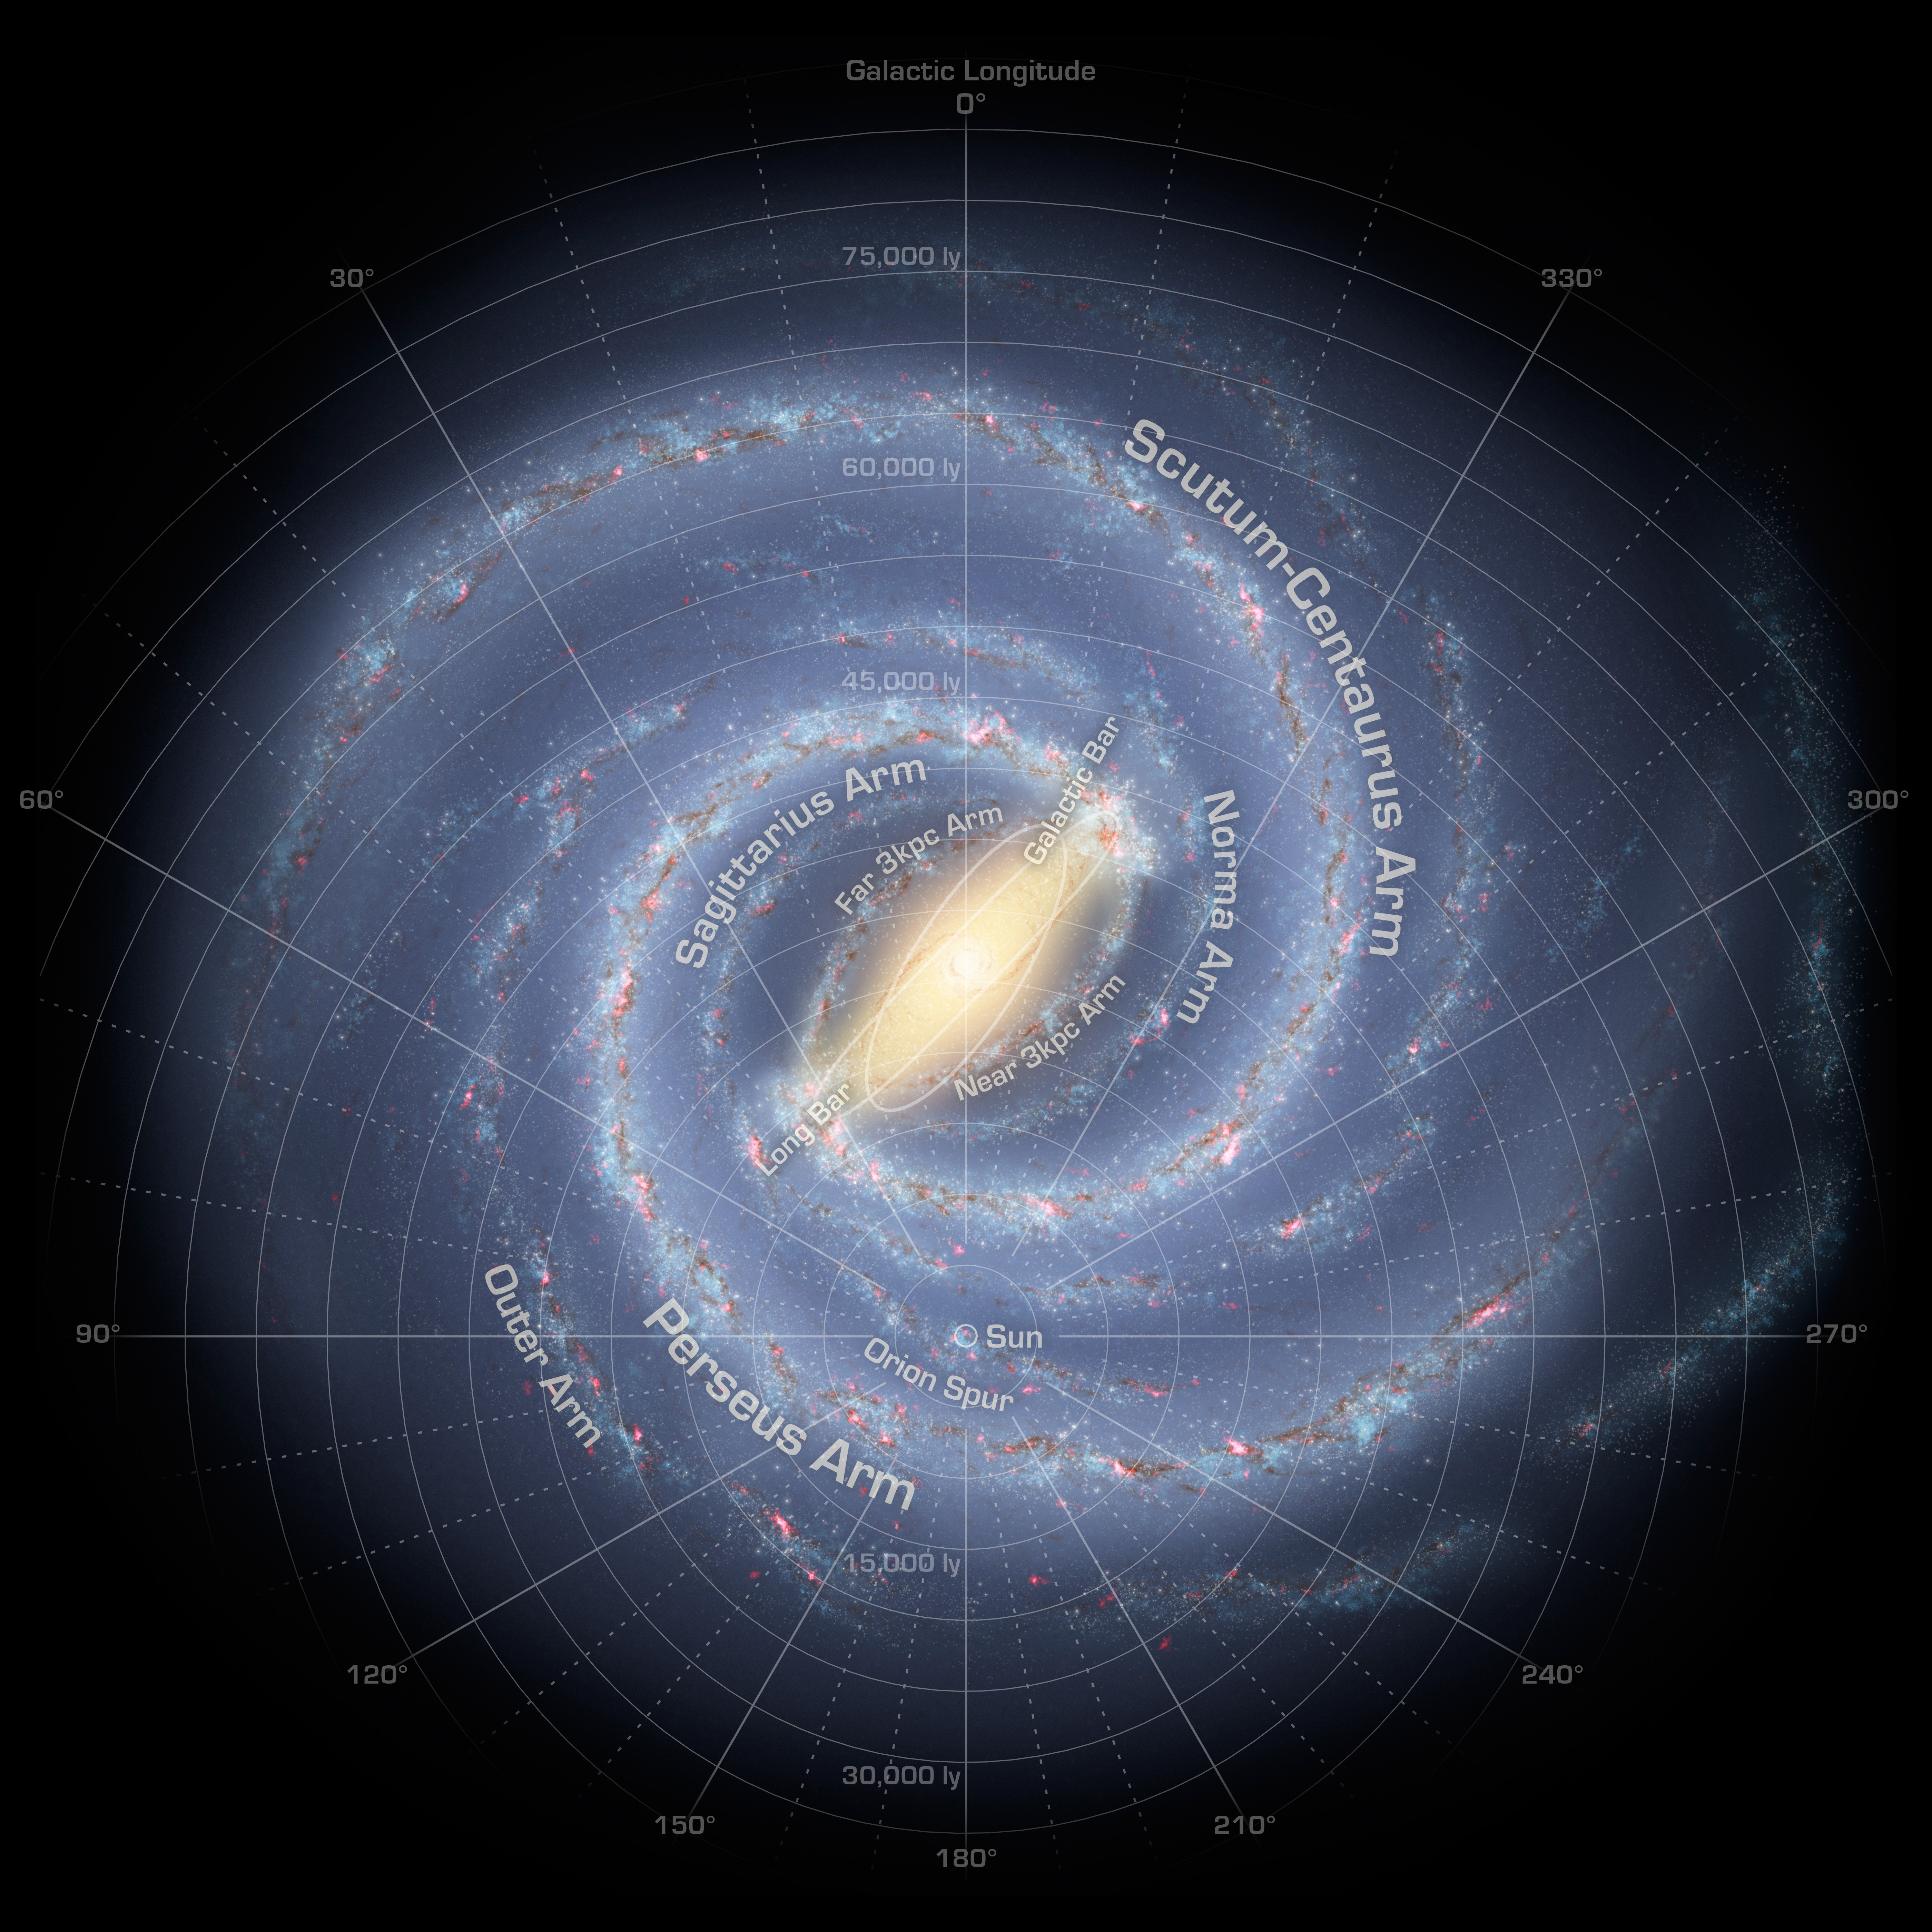
\includegraphics{figures/MWplaneAnnotated.jpg}}
\vskip 0.1in
\scalebox{0.37}{\hskip -2.8in \includegraphics{figures/snapshot1.jpg}}
\end{center}
\end{minipage}

\begin{minipage}[t]{14cm}
\begin{center}
\vskip -1in
{\large \color{red} Outer halo studies: RR Lyrae from SDSS Stripe 82}
\end{center}

\begin{itemize}
\item {\bf Top left:} the disk structure (artist's conception based on the Spitzer and
      other surveys of the Galactic plane)
\item {\bf Bottom left:} the halo density (multiplied by $R^3$; yellow and red are overdensities
      relative to mean $\rho(R)\propto R^{-3}$ density) as traced by RR Lyrae from SDSS Stripe 82
      (Sesar et al. 2010ab, ApJ 708, 717; ApJ 717, 133), compared in scale to the top panel
\item {\color{blue} Conclusions:} the spatial distribution of halo stars is highly
inhomogeneous (clumpy); when averaged, the stellar volume density decreases
as $\rho(R)\propto R^{-3}$ out to $\sim$30 kpc, and then becomes steeper.
\end{itemize}     

\end{minipage}}
\vfill 
\end{slide}
%------------------------------------------------------------------------------


%------------------------------------------------------------------------------

\begin{slide}

\begin{center}
\large \colour{red} Summary of SDSS Stellar Count Analysis 
\end{center}
\vskip -0.1in
\begin{itemize}
   \item 3D stellar number density maps of the Milky Way from SDSS  observations of 
         $\sim$50 million stars; analysis based on photometric distances and
         thus model-independent
   \item A two-component exponential disk model is in fair agreement with the data;
         halo properties, such as power-law index, poorly constrained due to
         rich substructure and limited sky coverage;
         however, an oblate halo is always preferred (no strong evidence for triaxial halo)
   \item A remarkable localized overdensity in the direction of Virgo over at least $\sim$2000 deg$^2$ 
         of the sky; steepening of the halo profile beyond $\sim$30 kpc
   \item {\color{red} \bf Clumps/overdensities/streams are an integral part of
         Milky Way structure, both of halo and the disk(s)}
\end{itemize}    
\vfill
\end{slide}



%------------------------------------------------------------------------------





\end{document}
